\documentclass[11pt, a4paper]{article}
\usepackage{polski}
\usepackage[utf8]{inputenc}
\usepackage{amsfonts}
\usepackage{amsmath}

\usepackage{caption}
\usepackage{subcaption}

\usepackage{graphicx}
\graphicspath{{./../img/}}

\usepackage{hyperref}
\hypersetup{
    colorlinks=true,
    linkcolor=blue,
    urlcolor=blue,
    pdftitle={Sprawozdanie},
    pdfpagemode=FullScreen,
    pdfauthor={Witold Karaś}
}
\usepackage{pgfplots}
\pgfplotsset{compat = newest}

\title{Sprawozdanie \\
\large Obliczenia naukowe - Lista 4\\}
\author{Witold Karaś}
\date{}
\begin{document}
\maketitle

\section{zadanie 1}
Zadanie polegało na implementacji funkcji obliczającej ilorazy różnicowe.

\subsection{Iloraz różnicowy: }
Jeśli \(f: X \rightarrow Y\) oraz \(x_0, x_1 \in X\) to ilorazem różnicowym nazywamy
\[\ f[x_0] = f(x_0)\]
\[\ f[x_0, x_1] = \frac{f(x_0) - f(x_1)}{x_0 - x_1}\]
Ponadto ilorazy różnicowe spełniają równość:
\[ f[x_0, x_1, \ldots, x_n] = \frac{f[x_1, x_2, \ldots, x_{n-1}] - f[x_0, x_1, \ldots, x_n]}{x_n - x_0} \]

Warto zauważyć że jeśli \(\Delta x = x_0 - x_1 \rightarrow 0 \) to iloraz różnicowy \(f[x_0, x_1]\) odpowiada wartości pochodnej pierwszego stopnia w punkcie \(x_0\).

\subsection{Opis algorytmu: }
Algorytm na wejściu dostaje wektory długości \(n + 1\) argumentów i wartości pewnej funkcji.\\ Wyjściem jest wektor ilorazów różnicowych, długości \(n + 1\), w postaci: 
\[ [f[x_0], f[x_0, x_1], \ldots,f[x_0, x_1, \ldots, x_{n - 1}], f[x_0, x_1, \ldots, x_n] ]\] 
Funkcja została oprogramowana bez użycia macierzy 2-wymiarowej. 
Aby to osiągnąć korzystamy z zagnieżdżonej pętli oraz z równości obliczania ilorazów różnicowych.

\begin{align*}
  f[x_0] &\searrow & & & & & f[x_0]\\
  f[x_1] & \begin{array}{c} \rightarrow \\ \searrow \end{array} &f[x_0, x_1]&\searrow & & & f[x_0, x_1]\\
  \vdots & & & &\cdots & &\vdots\\
  f[x_{n - 1}] &\begin{array}{c} \rightarrow \\ \searrow \end{array} &f[x_{n-2}, x_{n-1}] &\begin{array}{c} \rightarrow \\ \searrow \end{array} &\cdots &\begin{array}{c} \rightarrow \\ \searrow \end{array} &f[x_{0}, x_{1}, \ldots, x_{n-1}]\\
  f[x_n] &\rightarrow & f[x_{n-1}, x_{n}] & \rightarrow &\cdots &\rightarrow &f[x_{0}, x_{1}, \ldots, x_n]
\end{align*}


\section{zadanie 2}
Zadanie polegało na implementacji funkcji obliczającej wartość wielomianu interolacyjnego stopnia \(n\) w postaci Newtona w punkcie \(x = t\) za pomocą uogólionego algorytmu Hornera w czasie liniowym.\\
Algorytm na wejściu dostaje wektory długości argumentów \(n + 1\) oraz wektor ilorazów różnicowych.
Wyjściem jest wartość wielomianu w punkcie \(x = t\) 

\subsection{Opis algorytmu: }
Wartość wielomianu interpolacyjnego Newtona w punkcie jest równa:
\[N_n(x) = f[x_0] + f[x_0, x_1](x - x_0) + \ldots + f[x_0, x_1, \ldots, x_n](x - x_0)(x - x_1)\ldots(x - x_{n-1})\]
można ją obliczać za pomocą uogólnionego schematu Hornera
\begin{align*}
 w_n(x) & := & f[x_0, x_1, \ldots, x_n]&\\
 w_k(x) & := & f[x_0, x_1, \ldots, x_k] + (x - x_k)w_k(x)& \forall(k = n-1, \ldots, 0)\\
 N_n(x) & := & w_0(x) &\\
\end{align*}

Algorytm wykorzystuje jedną pętlę dlatego jego złożoność obliczeniowa wynosi \(O(n)\).
\section{zadanie 3}
Zadanie polegało na implementacji funkcji rozwiązującej równanie \(f(x) = 0\) metodą Eulera(siecznych). Polega ona na przybliżaniu dostatecznie małych odcinków funkcji za pomocą funkcji liniowej. 

\subsection{Opis algorytmu: }
Najpierw algorytm sprawdza oblicza \(f(a)\) oraz \(f(b)\). Następnie w pętli porównywane są wartości \(f(a)\) oraz \(f(b)\). W przypadku gdy \(f(a) > f(b)\) to \(a\) zamieniane jest z \(b\) oraz \(f(a)\) zamieniane jest z \(f(b)\). Obliczane jest nowe \(a\) oraz w miejscu przecięcia się siecznej z osią OX oraz nowe \(f(a)\). Sprawdzany jest warunek końca \(|b-a| < \delta\) lub \(|f(a)| < \epsilon\). W przeciwnym wypadku wykonywana jest kolejna iteracja. Metoda siecznych ma tę przewagę nad metodą Newtona że nie musimy znać pochodnej danej funkcji aby znaleźć przybliżenie pierwiastka funkcji.
\section{zadanie 4}
Zadanie polegało na instalacji pakietu \textbf{Polynomials} oraz wykorzystaniu jego funkcji do znalezienia miejsc zerowych wielomianu Wilkinsona w dwóch postaciach - naturalnej oraz iloczynowej:\\

\( P(x) = x^{20} - 210x^{19} + 20615x^{18} - 1256850x^{17} + 53327946x^{16} - 1672280820x^{15} + 40171771630x^{14} - 756111184500x^{13} + 11310276995381x^{12} - 135585182899530x^{11} + 1307535010540395x^{10} - 10142299865511450x^9 + 63030812099294896x^8 - 311333643161390640x^7 + 1206647803780373360x^6 - 3599979517947607200x^5 + 8037811822645051776x^4 - 12870931245150988800x^3 + 13803759753640704000x^2 - 8752948036761600000x^1 + 2432902008176640000x^0 \) \\
oraz
\[ p(x) = \prod_{i=1}^{20}(x-i)\]\\

\subsection{Wnioski:}
Oczywiście \(p(x) = P(x)\). Obliczone pierwiastki P(x) różnią się od spodziewanych wyników. Niewielka zmiana współłczynnika znacząco zmienia wyniki co implikuje, że zadanie jest źle uwarunkowane. Dokładność arytmetyki \textbf{Float64} ma 15-17 cyfr znaczących w systemie dziesiętnym. Wolny współczynnik wielomianu to \(20!\) i ma 19 cyfr znaczących co wykracza poza precyzję jaką dysponujemy.

\begin{table}
  \makebox[\textwidth]{
    \centering
    \begin{tabular}{|c|c|c|c|c|}
    \hline
    \emph{k} & \(z_k\) & \(|P(z_k)|\) & \(|p(z_k)|\) & \(|z_k - k|\)  \\
    \hline
    \hline
    1 & 0.9999999999996989 & 35696.50964788257 & 36720.50964788227 & 3.0109248427834245e-13 \\
    2 & 2.0000000000283182 & 176252.60026668405 & 192636.60026691604 & 2.8318236644508943e-11 \\
    3 & 2.9999999995920965 & 279157.6968824087 & 362101.69687113096 & 4.0790348876384996e-10 \\
    4 & 3.9999999837375317 & 3.0271092988991085e6 & 2.7649652999648857e6 & 1.626246826091915e-8 \\
    5 & 5.000000665769791 & 2.2917473756567076e7 & 2.2277473671348542e7 & 6.657697912970661e-7 \\
    6 & 5.999989245824773 & 1.2902417284205095e8 & 1.2769707122070245e8 & 1.0754175226779239e-5 \\
    7 & 7.000102002793008 & 4.805112754602064e8 & 4.780526156335614e8 & 0.00010200279300764947 \\
    8 & 7.999355829607762 & 1.6379520218961136e9 & 1.6337585675856934e9 & 0.0006441703922384079 \\
    9 & 9.002915294362053 & 4.877071372550003e9 & 4.870348427548107e9 & 0.002915294362052734 \\
    10 & 9.990413042481725 & 1.3638638195458128e10 & 1.362843071072106e10 & 0.009586957518274986 \\
    11 & 11.025022932909318 & 3.585631295130865e10 & 3.584087897760478e10 & 0.025022932909317674 \\
    12 & 11.953283253846857 & 7.533332360358197e10 & 7.531256581876213e10 & 0.04671674615314281 \\
    13 & 13.07431403244734 & 1.9605988124330817e11 & 1.9602984002587503e11 & 0.07431403244734014 \\
    14 & 13.914755591802127 & 3.5751347823104315e11 & 3.574748406282602e11 & 0.08524440819787316 \\
    15 & 15.075493799699476 & 8.21627123645597e11 & 8.215740477766903e11 & 0.07549379969947623 \\
    16 & 15.946286716607972 & 1.5514978880494067e12 & 1.5514314565843672e12 & 0.05371328339202819 \\
    17 & 17.025427146237412 & 3.694735918486229e12 & 3.6946500070912217e12 & 0.025427146237412046 \\
    18 & 17.99092135271648 & 7.650109016515867e12 & 7.650001670877033e12 & 0.009078647283519814 \\
    19 & 19.00190981829944 & 1.1435273749721195e13 & 1.14351402511197e13 & 0.0019098182994383706 \\
    20 & 19.999809291236637 & 2.7924106393680727e13 & 2.7923942556843e13 & 0.00019070876336257925 \\
    \hline
    \end{tabular}
    }
    \caption{wartości z wyjścia programu \textbf{zadanie4.jl, b)}}

\end{table}

\begin{table}[th]
  \makebox[\textwidth]{
    \centering
    \begin{tabular}{|c|c|c|c|}
    \hline
    \emph{k} & \(z_k\) & \(|P'(z_k)|\) & \(|z_k - k|\) \\
    \hline
    \hline
    1 & 0.9999999999998357 + 0.0im & 20259.872313418207 & 1.6431300764452317e-13 \\
    2 & 2.0000000000550373 + 0.0im & 346541.4137593836 & 5.503730804434781e-11 \\
    3 & 2.99999999660342 + 0.0im & 2.2580597001197007e6 & 3.3965799062229962e-9 \\
    4 & 4.000000089724362 + 0.0im & 1.0542631790395478e7 & 8.972436216225788e-8 \\
    5 & 4.99999857388791 + 0.0im & 3.757830916585153e7 & 1.4261120897529622e-6 \\
    6 & 6.000020476673031 + 0.0im & 1.3140943325569446e8 & 2.0476673030955794e-5 \\
    7 & 6.99960207042242 + 0.0im & 3.939355874647618e8 & 0.00039792957757978087 \\
    8 & 8.007772029099446 + 0.0im & 1.184986961371896e9 & 0.007772029099445632 \\
    9 & 8.915816367932559 + 0.0im & 2.2255221233077707e9 & 0.0841836320674414 \\
    10 & 10.095455630535774 - 0.6449328236240688im & 1.0677921232930157e10 & 0.6519586830380407 \\
    11 & 10.095455630535774 + 0.6449328236240688im & 1.0677921232930157e10 & 1.1109180272716561 \\
    12 & 11.793890586174369 - 1.6524771364075785im & 3.1401962344429485e10 & 1.665281290598479 \\
    13 & 11.793890586174369 + 1.6524771364075785im & 3.1401962344429485e10 & 2.0458202766784277 \\
    14 & 13.992406684487216 - 2.5188244257108443im & 2.157665405951858e11 & 2.518835871190904 \\
    15 & 13.992406684487216 + 2.5188244257108443im & 2.157665405951858e11 & 2.7128805312847097 \\
    16 & 16.73074487979267 - 2.812624896721978im & 4.850110893921027e11 & 2.9060018735375106 \\
    17 & 16.73074487979267 + 2.812624896721978im & 4.850110893921027e11 & 2.825483521349608 \\
    18 & 19.5024423688181 - 1.940331978642903im & 4.557199223869993e12 & 2.4540214463129764 \\
    19 & 19.5024423688181 + 1.940331978642903im & 4.557199223869993e12 & 2.0043294443099486 \\
    20 & 20.84691021519479 + 0.0im & 8.756386551865696e12 & 0.8469102151947894 \\
    \hline
    \end{tabular}
    }
  \caption{wartości z wyjścia programu \textbf{zadanie4.jl, b)}}
\end{table}

\section{zadanie 5}
Zadanie polegało na przeprawadzeniu eksperymentów dla funkcji rekurencyjnej:
\[ p_{n+1} := p_n + rp_n(1-p_n), \textrm{dla } n = 0,1,2,...\]
dla danych początkowych \(p_0 = 0.01, r=3\) oraz 40 iteracji. 
W części \textbf{a)} rekurencja została podzielona na 4 interwały takie że po każdym stosowane było obięcie do 3 miejsc po przecinku, obliczenia wykonywane były we \texttt{Float32}. W części \texttt{b)} program obliczał tą samą rekurencję w precyzji \texttt{Float32} i \texttt{Float64}.
\subsection{Wnioski:}
Wyniki w tabeli wskazują jak ważna jest dokładność z jaką reprezentowane są liczby.
\begin{table}[ht]
  \makebox[\textwidth]{
    \centering
    \begin{tabular}{|c|c|}
    \hline
    \texttt{Float32}, 4*10 iteracji z obcięciem & \texttt{Float32} 40 iteracji  \\
    0.715 & 0.25860548 \\
    \hline
    \hline
    \texttt{Float32} 40 iteracji & \texttt{Float64} 40 iteracji  \\
    0.25860548 & 0.011611238029748606 \\
    \hline
    
    \end{tabular}
    }
    \caption{wartości z wyjścia programu \texttt{zadanie5.jl}}

\end{table}
\section{zadanie 6}

\subsection{Wyniki:}
Zadanie polegało na przetestowaniu funkcji /(rysujNnfx/) przygotowanej na potrzeby wcześniejszego zadania. Testy zostały wykonane na następujących danych wejściowych:
\begin{enumerate}
  \item \(f(x) = |x|; [a, b] = [-1, 1], n = 5, 10, 15 \)
  \item \(f(x) = \frac{1}{1 + x^2}; [a, b] = [-5, 5], n = 5, 10, 15 \)
\end{enumerate}

\begin{figure}[t]
  \centering
  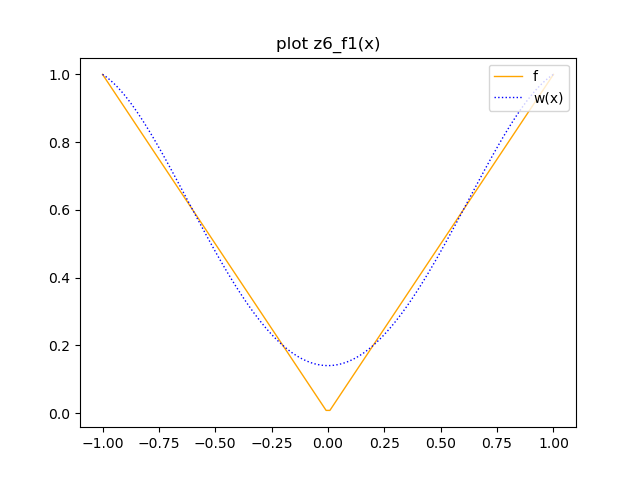
\includegraphics[width=\textwidth]{plot_z6_f1(x)_5.png}
  \caption{Wykres funkcji \(f(x) = |x|, n = 5\)}
\end{figure}

\begin{figure}[t]
  \centering
  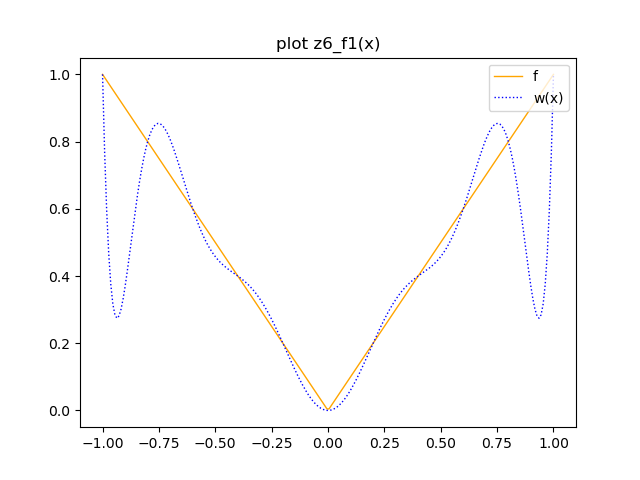
\includegraphics[width=\textwidth]{plot_z6_f1(x)_10.png}
  \caption{Wykres funkcji \(f(x) = |x|, n = 10\)}
\end{figure}

\begin{figure}[t]
  \centering
  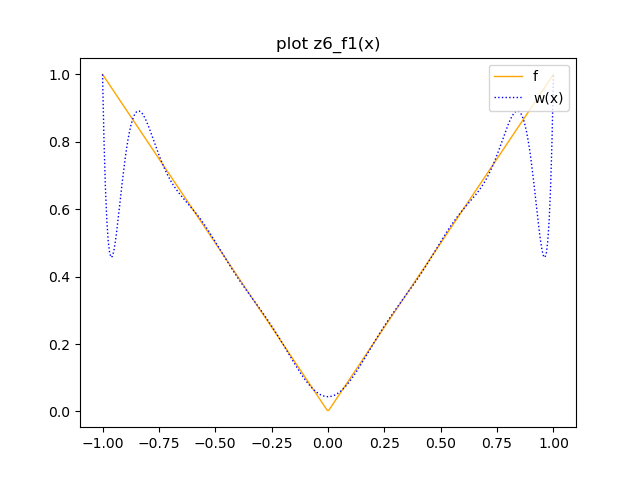
\includegraphics[width=\textwidth]{plot_z6_f1(x)_15.png}
  \caption{Wykres funkcji \(f(x) = |x|, n = 15\)}
\end{figure}

\begin{figure}[t]
  \centering
  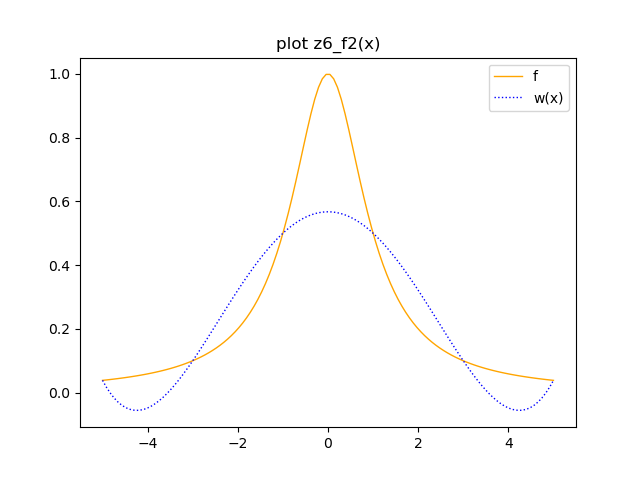
\includegraphics[width=\textwidth]{plot_z6_f2(x)_5.png}
  \caption{Wykres funkcji \(f(x) = \frac{1}{1+x^2}, n = 5\)}
\end{figure}

\begin{figure}[t]
  \centering
  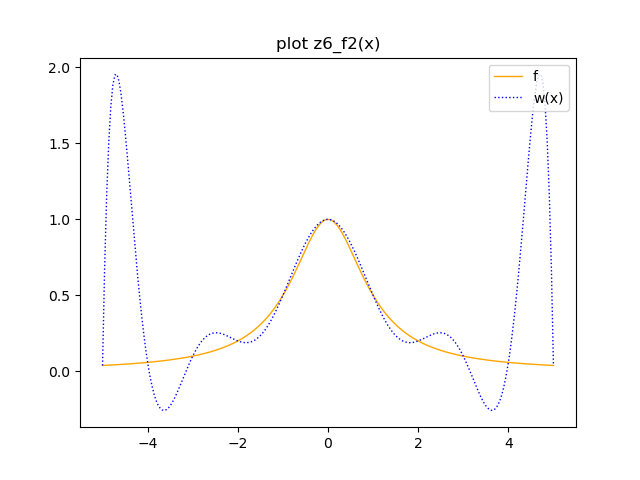
\includegraphics[width=\textwidth]{plot_z6_f2(x)_10.png}
  \caption{Wykres funkcji \(f(x) = \frac{1}{1+x^2}, n = 10\)}
\end{figure}

\begin{figure}[t]
  \centering
  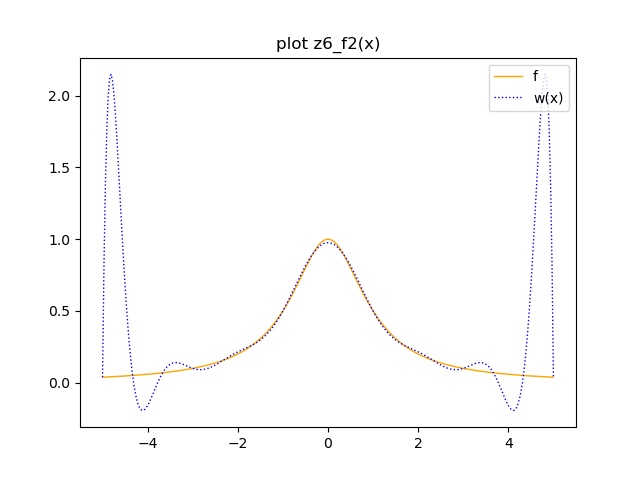
\includegraphics[width=\textwidth]{plot_z6_f2(x)_15.png}
  \caption{Wykres funkcji \(f(x) = \frac{1}{1+x^2}, n = 15\)}
\end{figure}

\subsection{Wnioski:}
Dla testowanych funkcji przybliżenia niezbyt wiernie oddają spodziewane kształty.
W tych przypadkach możemy zaobserwować efekt Rungego. Jest to zjawisko polegające na pogorszeniu się jakości interpolacji mimo zwiąkszenia liczby jej węzłów co jest efektem odwrotnym do zamierzonego. Efekt jest wywołany przez równomierne rozłożenie węzłów interpolacji. Można go uniknąć kładąc więcej węzłów interpolacji na końcach przedziału.

\end{document}